\documentclass[a4paper,12pt]{article}
\usepackage[polish]{babel}
\usepackage{polski}
\usepackage[utf8]{inputenc}
\usepackage[T1]{fontenc}
\usepackage[margin=1.5cm]{geometry}
\usepackage{longtable}
\usepackage{graphicx}
\usepackage{float}
\usepackage{pdfpages}


\title{Wizualizacja danych sonaru}
\author{Dorian Janiak}
\date{11.06.2015}

\begin{document}

\maketitle

\section{Krótki opis}
Projekt zakładał stworzenie aplikacji komputerowej, która będzie wizualizowała
otrzymywane dane z sonaru ultradźwiękowego. Aplikacja ma próbować łączyć dane
w taki sposób, aby móc z nich stworzyć zarys otoczenia. Drugą część projektu
stanowi symulacja, której zadaniem jest z odpowiednio przygotowanych obiektów
geometrycznych wygenerować dane potrzebne do wykonania wizualizacji 
(ma być symulacją sonaru). 
Dane mają zostać przesłane przy pomocy wybranego protokołu komunikacyjnego.

\section{Cel}
Celem projektu było zapoznanie się ze środowiskiem Qt oraz sposobami wizualizacji danych przy użyciu jego klas.
Jednym z problemów, który został również poruszony w ramach pracy był 
sposób komunikacji modułów i przesył danych. Jednym z ważnych powodów podjęcia się realizacji tego tematu była chęć głębszego poznania biblioteki OpenGL. 




\section{Opis projektu}
Projekt składał się z dwóch części. Pierwsza polegała na stworzeniu aplikacji głównej dla komputerów PC przy użyciu środkowiska Qt. Druga polegała na stworzeniu aplikacji symulującej robota uruchamianej na telefonie z systemem Android.

\subsection{Aplikacja główna}
Aplikacja główna powstała w środowisku Qt. Pozwala ona użytkownikowi na połączenie się z robotem lub symulatorem, a następnie sterowanie nim. Połączenie ustanawiane jest przy użyciu obiektu klasy QSerialPort, który obsługuje \textbf{port szeregowy}. Po połączeniu się z urządzeniem możliwe są trzy operacje:
\begin{itemize}
\item przemieszczenie robota,
\item kalibracja silnika krokowego (zmiana kąta akustycznego sonaru)
\item wykonanie skanowania otoczenia
\end{itemize} 
Status wykonywanych operacji publikowany jest w oknie logów. Dzięki temu użytkownik dowiaduje się czy ustanowiono połączenie i z jakim portem oraz czy operacje, których wykonania zażądał rzeczywiście się wykonały.\newline
Rezultaty skanowania otoczenia przedstawiane są w głównym oknie aplikacji komputerowej. Wizualizowane są przy użyciu odziedziczonych klas QOpenGLWidget oraz QOpenGLFunctions, które obsługują bibliotekę \textbf{OpenGL}. \newline

\subsection{Symulator robota}
Aplikacja symulująca robota powstała w środowisku Android Studio i przeznaczona jest na telefony komórkowe z systemem Android w wersji nie niższej niż 2.3 . Aplikacja pozwala na załadowanie pliku OBJ zawierającego mapę otoczenia. Następnie po naciśnięciu przycisku 'Zasymuluj' otrzymywane są rezultaty skanowania otoczenia z zadanej pozycji robota. Skanowanie otoczenia odbywa się najprostszą metodą (poprzez prowadzenie prostych linii i sprawdzanie przecięć z krawędziami). \newline
W ramach projektu symulator miał komunikować się z komputerem. Niestety nie udało mi się tego zrealizować. W trakcie realizacji projektu skupiłem się na tym, aby aplikacja komputerowa zadziałała z robotem. Ponieważ z robotem można się komunikować jedynie przy użyciu portu szeregowego, a udało mi się znaleźć informacje według, których telefon również można połączyć z komputerem PC poprzez port szeregowy, postanowiłem skorzystać z klasy QSerialPort zamiast QtBluetooth. Jest to rzeczywiście możliwe, ale w trakcie realizacji projektu okazało się, że oba modele telefonów, na których mogłem testować symulator \textbf{nie posiadają funkcji SPP}, która właśnie odpowiada za możliwość takiego łączenia urządzenia z komputerem PC. \newline
\subsubsection{Możliwe rozwiązania}
Ponieważ nie udało mi się rozwiązać problemu ze względu na ograniczenia czasowe, postanowiłem znaleźć możliwe rozwiązania:
\begin{itemize}
\item Pierwsze rozwiązanie polega na stworzeniu dodatkowego modułu w aplikacji głównej, który dziedziczy po klasie \textbf{QtBluetooth} i stworzeniu komunikacji na zasadzie serwer-klient. Zaletą rozwiązania jest zachowanie spójności części projektu przeznaczonej na PC, jednak można liczyć się z pogorszeniem czytelności zarówno GUI aplikacji jak i jej implementacji.
\item Drugie rozwiązanie polega na stworzeniu drugiej aplikacji komputerowej, która jedynie łączy się poprzez Bluetooth z urządzeniem i przekierowuje odbierane i wysyłane dane na wirtualny port szeregowy. Rozwiązanie nie zachowuje spójności części projektu przeznaczonej na PC, ponieważ użytkownik zmuszony byłby do uruchamiania obu aplikacji oraz symulatora. Zaletą natomiast jest fakt, że zachowana byłaby czytelność głównej aplikacji komputerowej.
\item Trzecie rozwiązanie polega na stworzeniu symulatora na komputerze PC tak jak to było w pierwotnych założeniach projektu i wysyłanie danych poprzez wirtualny port szeregowy. 
\item Czwarte rozwiązanie polega na znalezieniu telefonu z SPP oraz dokończeniu symulatora robota. 
\end{itemize}
Najbardziej racjonalne rozwiązania wydają się \textbf{pierwsze i trzecie}, natomiast najmniej czwarte. To ostatnie odpada, ponieważ wiąże się to z nakładami finansowymi. Poza tym w takiej sytuacji użytkownikowi należałoby narzucić wymóg posiadania telefonu z funkcją SPP, a to zniechęciłoby potencjalnych zainteresowanych do korzystania z aplikacji. 
\subsection{Robot}
Robot powstał w ramach projektu z kursu Roboty Mobilne. Jednak na nim znajduje się gotowa aplikacja, która jest w stanie przeskanować otoczenie oraz zasymulować jazdę robota. Aplikacja główna bardzo dobrze współpracuje z rzeczywistym robotem. Dzięki zastosowaniu modułu Bluetooth HC-05 robot komunikuje się z komputerem PC bezprzewodowo, a mimo to połączenie widziane jest jako połączenie szeregowe.  



\section{Funkcjonalność}
\subsection{Funkcjonalność skończona}
Poniżej zamieszczona została lista funkcjonalności, którą udało się ukończyć w ramach projektu. 
\subsubsection{Aplikacja na komputerze PC}
\begin{itemize}
\item Rysowanie na scenie 3D mapy otoczenia.
\item Wczytywanie danych pomiarowych sonaru z pliku (w przypadku symulacji).
\item Łączenie nowo odczytanej z poprzednio odczytaną mapą terenu. 
\item Możliwość sterowania widokiem 3D (rotacja oraz translacja).
\item Wyświetlanie logów dotyczących przesyłanych komunikatów oraz interpretacja występujących błędów.
\item Rysowanie na scenie 3D robota załadowanego z pliku STL.
\item Udostępnienie pilota pozwalającego na sterowanie robotem (lub symulacją).
\item Udostępnienie okna konfiguracji portów COM połączenia szeregowego.
\item Połączenie z portem szeregowym oraz obsługa komunikacji.
\item Wysłanie żądania i weryfikacja wiadomości zwrotnej \textbf{przemieszczenia robota}
\item Wysłanie żądania i weryfikacja wiadomości zwrotnej \textbf{skanowania otoczenia}
\item Wysłanie żądania i weryfikacja wiadomości zwrotnej \textbf{zmiany kąta akustycznego czujnika}
\end{itemize}
\subsubsection{Symulator na urządzeniu}
\begin{itemize}
\item Ładowanie plików OBJ, parsowanie oraz raportowanie wczytanych informacji
\item Wykonanie skanowania otoczenia przy użyciu bardzo prostego algorytmu oraz wyświetlenie wyników skanowania.
\item Nawiązanie połączenia Bluetooth z komputerem PC.
\end{itemize}

\subsection{Funkcjonalność nieskończona}
Poniżej zamieszczone została lista funkcjonalności, których nie udało się ostatecznie wykonać.
\subsubsection{Symulator na urządzeniu}
\begin{itemize}
\item Wysłanie danych do aplikacji wizualizującej poprzez interfejs komunikacyjny (Bluetooth)
\item Odbieranie żądania przemieszczenia robota na scenie i przesłanie wyniku operacji
\item Odbieranie żądania wykonania symulacji i przesłania wyników operacji
\end{itemize}


\section{Protokół komunikacji}
Na potrzeby realizacji projektu powstał protokół komunikacji, bazujący na poniższych typach wiadomości:
\begin{itemize}
\item Potwierdzenie powodzenia operacji. 
\begin{verbatim}
	W0;0
\end{verbatim}
\item Informacja o rozpoczęciu działania robota.
\begin{verbatim}
	W1;0
\end{verbatim}
\item Żądanie wykonania skanowania wysyłane do robota.
\begin{verbatim}
	W2;2;ile_pomiarów;vKąt
\end{verbatim}
	\begin{itemize}
	\item ile\_pomiarów - całkowita liczba dodatnia, ilość pomiarów jakie mają zostać wykonane w zakresie 180 stopni obrotu.
	\item vKąt - całkowita liczba dodatnia, szybkość obrotu czujnika wyrażona w stopniach na sekundę.
	\end{itemize}
\item Rezultat wykonania skanowania, który robot wysyła w odpowiedzi na wiadomość W2.
\begin{verbatim}
	W3;ile_pomiarów*2;[kąt_akustyczny;pomiar_w_cm]
\end{verbatim}
	\begin{itemize}
	\item ile\_pomiarów - całkowita liczba dodatnia, ilość pomiarów jakie zostały wykonane w ramach jednego pomiaru. 
	\item kąt\_akustyczny - całkowita liczba dodatnia, kąt wyrażony w stopniach
	\item pomiar\_w\_cm - całkowita liczba dodatnia, wynik pomiaru wyrażony w cm.
	\end{itemize}
\item Żądanie obrotu wału silnika krokowego bez wykonania pomiarów. Odpowiedzią na pozytywne wykonanie operacji jest wiadomość W0.
\begin{verbatim}
	W4;3;kierunek;kąt;vKąt
\end{verbatim}
	\begin{itemize}
	\item kierunek - 1 gdy zgodnie zasadą prawej dłoni, w przeciwnym wypadku 0
	\item kąt - całkowita liczba, kąt obrotu wyrażony w stopniach
	\item vKąt - całkowita liczba dodatnia, szybkość obrotu czujnika wyrażona w stopniach na sekundę.
	\end{itemize}
\item Żądanie jazdy robota, a konkretniej przemieszczenia do konkretnego punktu. Najpierw robot powinien obrócić się o kąt zadany w parametrze obrót\_przed\_ruchem, następnie przejechać po linii prostej odległość podaną w parametrze dystans\_cm, a na koniec jeszcze obrócić się o kąt podany w parametrze obrót\_po\_ruchu. 
\begin{verbatim}
	W5;4;vSzybkość;dystans_cm;obrót_przed_ruchem;obrót_po_ruchu
\end{verbatim}
	\begin{itemize}
	\item vSzybkość - całkowita liczba dodatnia, szybkość wyrażona w cm na sekundę
	\item dystans\_cm - całkowita liczba dodatnia, dystans jaki ma robot przejechać po linii prostej wyrażony w cm
	\item obrót\_przed\_ruchem - całkowita liczba, kąt wyrażony w stopniach
	\item obrót\_po\_ruchu - całkowita liczba, kąt wyrażony w stopniach
	\end{itemize}
\item Rezultat wykonania przemieszczenia robota, który jest odpowiedzią na wiadomość W5.  
\begin{verbatim}
	W6;3;dystans_cm;obrót_przed_ruchem;obrót_po_ruchu
\end{verbatim}
	\begin{itemize}
	\item dystans\_cm - całkowita liczba dodatnia, dystans jaki ma robot przejechać po linii prostej wyrażony w cm
	\item obrót\_przed\_ruchem - całkowita liczba, kąt wyrażony w stopniach
	\item obrót\_po\_ruchu - całkowita liczba, kąt wyrażony w stopniach
	\end{itemize}
\item Niepowodzenie operacji.
\begin{verbatim}
	W99;0
\end{verbatim}
\end{itemize}


\section{Wygląd aplikacji}
\subsection{Aplikacja główna}
Główna aplikacja komputerowa składa się z widżetów oraz dodatkowych okien wyświetlanych w przypadku reakcji na błędy lub wywołanie akcji z poziomu paska menu.
\subsubsection{Widżety dokowane}
Aplikacja składa się z głównego okna widocznego na rysunku \ref{app2}.
\begin{figure}
\centering
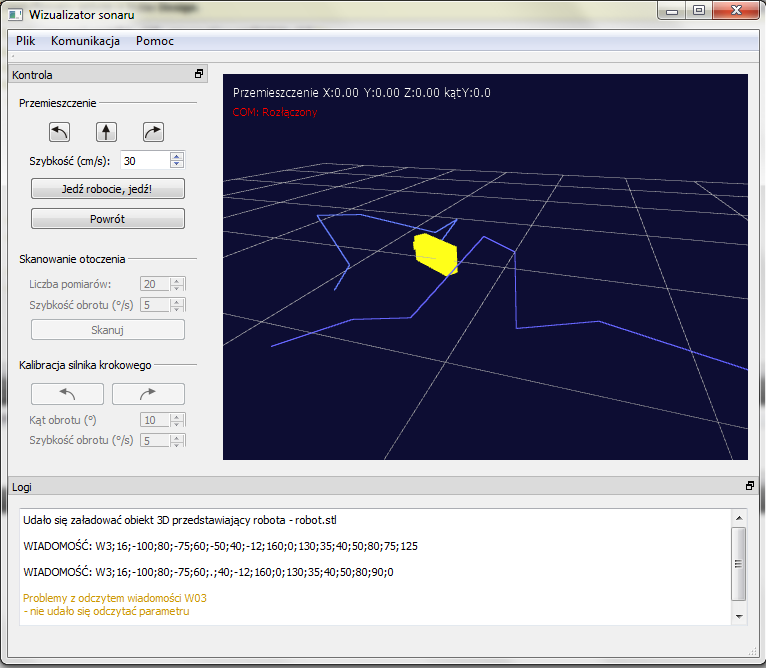
\includegraphics[width=\linewidth]{app2.png}
\caption{Wygląd aplikacji}
\label{app2}
\end{figure}
\begin{figure}[p]
\centering
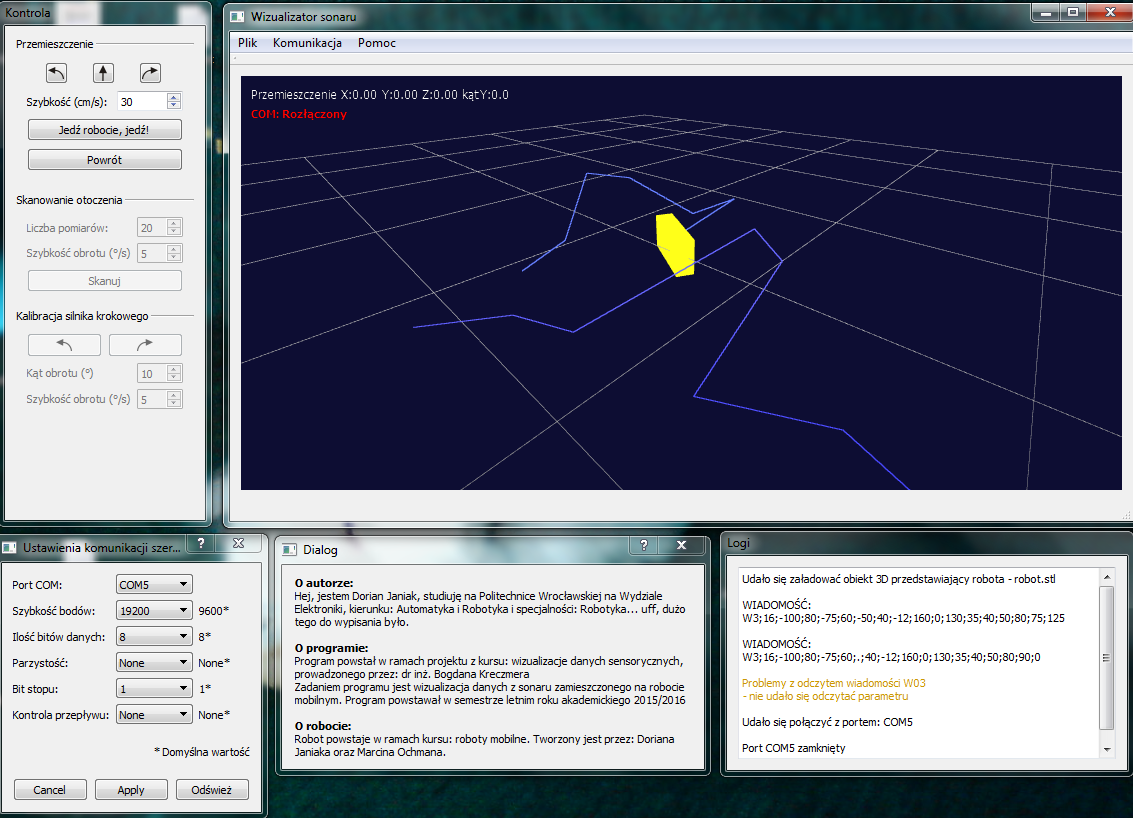
\includegraphics[width=\textheight, angle=90]{app5.png}
\caption{Otwarte kilka okien oraz widżetów - otwieranie na kilku monitorach}
\label{app5}
\end{figure}
W oknie znajdują się trzy widżety: Kontrola, Logi oraz widok 3D. Oba pierwsze widżety są dokowane i mogą zostać odłączone. Pozwala to na wygodniejsze operowanie lub nawet rozkładanie widoku aplikacji na kilka monitorów (rysunek \ref{app5} ). Widżet \textbf{Logi} zawiera jedynie pole tekstowe, którego edytować nie można i w którym pojawiają się wszelkie informacje na temat statusu operacji oraz aplikacji. Zostały wyróżnione różnego typu komunikaty:
\begin{itemize}
\item kolor czarny - zwykła informacja
\item kolor pomarańczowy - ostrzeżenie
\item kolor czerwony - błąd (ale nie krytyczny)
\end{itemize}
Widżet \textbf{Kontrola} składa się z grup:
\begin{itemize}
\item Przemieszczenie - gdzie udostępnione zostały trzy przyciski do sterowania pozycją robota w jakiej chcielibyśmy, aby ostatecznie się znalazł. Aby nakazać robotowi przemieszczenie się do zadanej pozycji należy nacisnąć przycisk \textit{Jedź robocie, jedź!} (Choć należałoby się zastanowić czy przycisk nie powinien nazywać się \textit{Robocie, niech ktoś cię przesunie!} w kontekście niezamontowanych kół do robota). W przeciwnym wypadku robot się nie znajdzie w zadanej pozycji i przy najbliższym skanowaniu otoczenia lub przy naciśnięciu przycisku \textit{Powrót} robot powróci do ostatniej zapamiętanej pozycji (takiej, do której miał dojechać). Można zadać również szybkość jazdy robota. Robot nie musi jej obsłużyć.
\item Skanowanie otoczenia - grupa pozwala na nakazanie robotowi wykonania skanu otoczenia. Skanowanie odbywa się w zakresie 90 do -90 stopni. Można zadać ile pomiarów ma się znaleźć w ramach jednego skanowania i z jaką szybkością ma się wykonywać skanowanie (obrót silnika krokowego). Aby grupa była dostępna aplikacja musi połączyć się z robotem. 
\item Kalibracja silnika krokowego - grupa pozwala na obrócenie silnika krokowego (sterowanie kątem akustycznym czujnika odległościowego) bez wykonywania pomiaru i odczytu mapy otoczenia. Aby grupa była dostępna aplikacja musi połączyć się z robotem.
\end{itemize}

\subsubsection{Widok 3D}
Główną część okna stanowi \textbf{widok 3D}, w którym przy użyciu myszy komputerowej można sterować kątem kamery (LPM + ruch), jej przybliżeniem (rolka) oraz przemieszczeniem jej centralnego punktu (PPM + ruch). W oknie tym rysowana jest mapa 3D.
 Widok jest renderowany przy użyciu klas \textbf{QOpenGLWidget} (od wersji Qt 5.4 wyparła QGLWidget) oraz \textbf{QOpenGLFunctions}, obsługujących OpenGL. W oknie pojawiają się takie obiekty jak:
\begin{itemize}
\item wyniki skanowania - widoczne na screenie (linie w odcieniach niebieskiego). Każdy dodatkowy pomiar jest podnoszony względem poprzedniego (wzdłuż osi Y) oraz jest rozjaśniany jego kolor. Pozwala to odróżnić kolejne pomiary od siebie. Jest to w szczególności przydatne gdy okaże się, że w trakcie jednego skanowania zostanie zarejestrowany pomiar bardziej odległy niż 3m - wtedy program odrzuca taki pomiar i siatka zostaje rozerwana w tym miejscu. Wtedy mimo kilku osobnych podsiatek można zauważyć, że pochodzą one z tego samego pomiaru, ponieważ są na jednakowej wysokości oraz o jednakowym kolorze.
\item robot - robot jest symbolizowany przez żółty obiekt. W praktyce można jednak obiekt ten zmienić poprzez podmianę pliku \textbf{objects/robot.stl}.
\item siatka - domyślnie jedna kratka odpowiada kwadratowi o boku 1 metru. 
\end{itemize}

\subsubsection{Dodatkowe okna}
Poważniejsze błędy, wymagające uwagi użytkownika są raportowane okienkiem błędu. 
\begin{figure} [H]
\centering
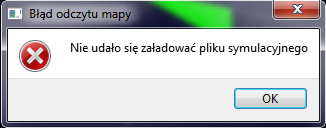
\includegraphics{error_screen.png}
\caption{Komunikat błędu}
\label{error_screen}
\end{figure}
Po wybraniu odpowiedniej opcji z paska menu otwiera się okno z informacjami o autorstwie.
\begin{figure} [H]
\centering
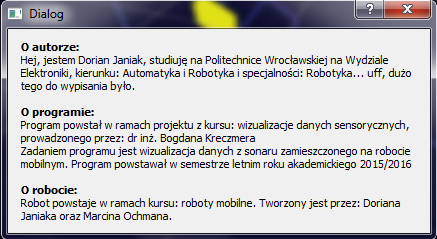
\includegraphics{app4.png}
\caption{Informacje o autorze i projektach}
\label{app4}
\end{figure}
Po wybraniu opcji \textit{Konfiguracja} z menu \textit{Komunikacja} wyświetla poniżej przedstawione okno konfiguracji połączenia szeregowego. 
\begin{figure} [H]
\centering
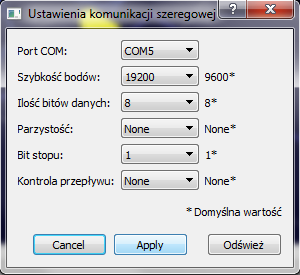
\includegraphics{app3.png}
\caption{Konfiguracja połączenia szeregowego}
\label{app3}
\end{figure}
Po wybraniu opcji \textit{Wyświetl informacje} z menu \textit{Komunikacja} wyświetla się poniższe okno z podsumowaniem aktualnie ustawionych parametrów komunikacji poprzez port szeregowy. 
\begin{figure} [H]
\centering
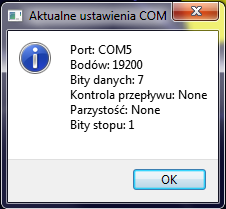
\includegraphics{app6_small.png}
\caption{Aktualnie ustawiona konfiguracja połączenia szeregowego}
\label{app6}
\end{figure}

\subsection{Symulator}
Symulator nie został ostatecznie połączony poprzez Bluetooth z komputerem, a więc nie pełni swojej funkcji. Jednak mimo to powstał już wstępny prosty intefejs graficzny, który pozwala na wczytywanie danych wejściowych i wyświetlenie wyniku skanowania.
\newline
Poniższy screen przedstawia ikonę aplikacji w menu Android na telefonie Sony Xperia U.
\begin{figure} [H]
\centering
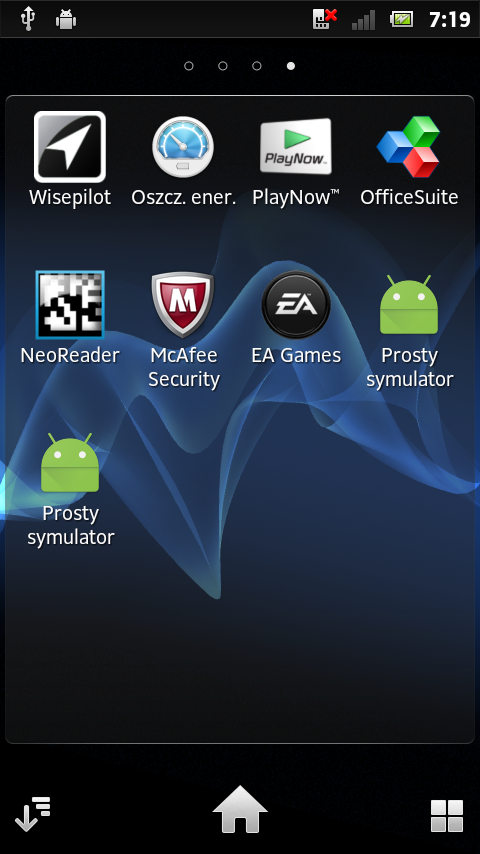
\includegraphics[height=300px]{s1.png}
\caption{Menu Android z aplikacją Prosty symulator}
\label{s1}
\end{figure}
Okno aplikacji po załadowaniu pliku z mapą otoczenia przedstawia się następująco:
\begin{figure} [H]
\centering
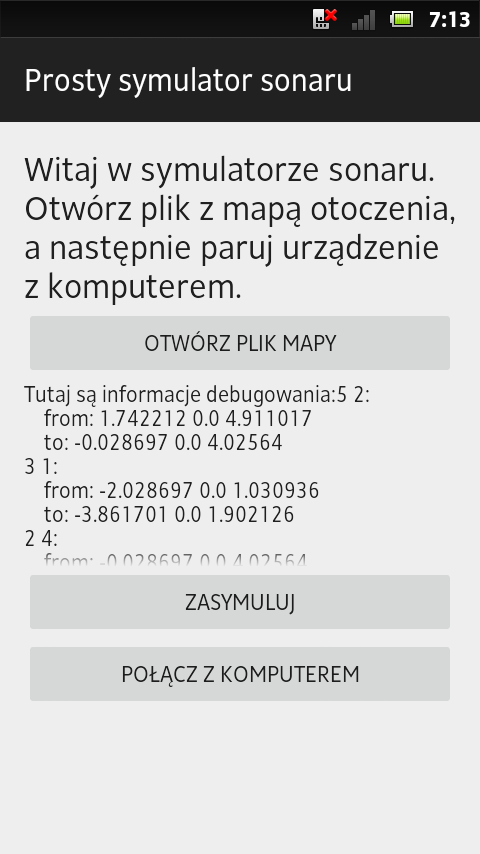
\includegraphics[height=300px]{s4.png}
\caption{Załadowana mapa otoczenia}
\label{s4}
\end{figure}
Aby załadować mapę otoczenia należy nacisnąć przycisk \textit{Otwórz plik mapy}. W takiej sytuacji otworzy się okno (Intent) wyboru pliku OBJ, które zostało stworzone przez Alexandra Ponomarev'a. 
\begin{figure} [H]
\centering
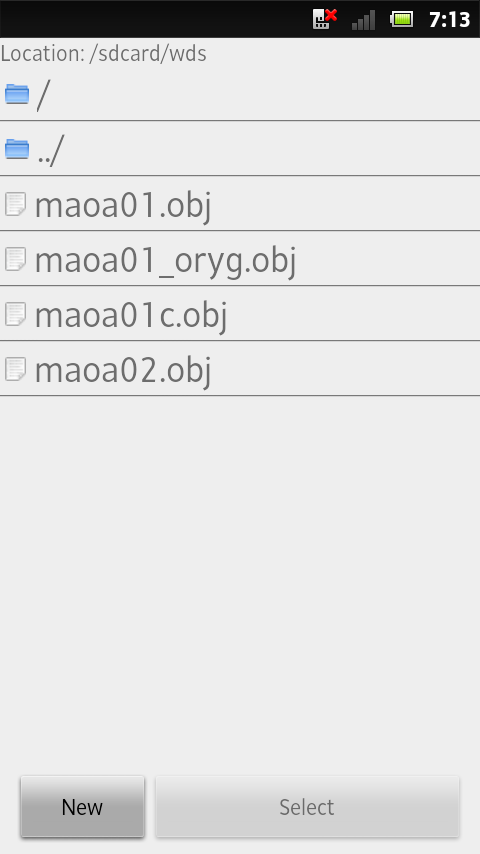
\includegraphics[height=300px]{s3.png}
\caption{Wybór pliku OBJ}
\label{s3}
\end{figure}
Natomiast po wciśnięciu przycisku \textit{Zasymuluj} zostanie obliczony symulowany wynik skanowania i zaprazentowany tak jak w poniższym oknie:
\begin{figure} [H]
\centering
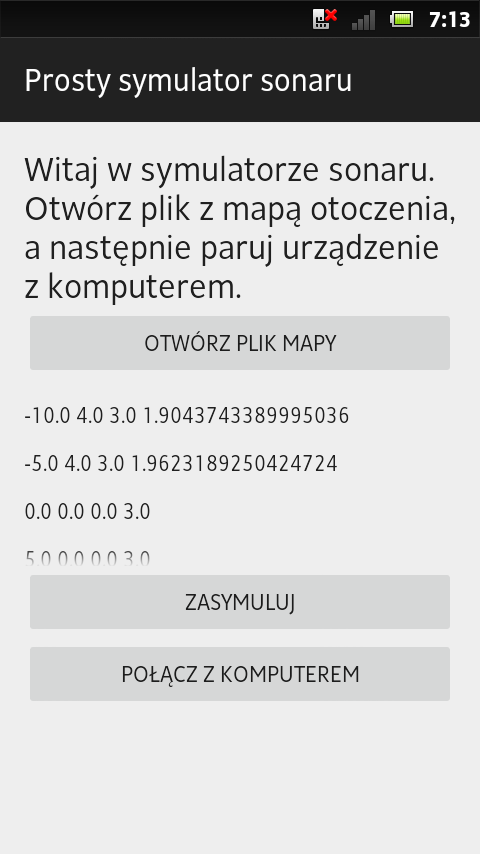
\includegraphics[height=300px]{s5.png}
\caption{Wynik symulacji}
\label{s5}
\end{figure}

\section{Diagramy}
Poniżej zaprezentowany został diagram klas dla głównej aplikacji komputerowej. 
Analizę należy rozpocząć od klasy textbf{MainWindow}, która odpowiada głównemu oknu aplikacji. Przechowuje ona obiekty pozostałych klas. 
\textbf{MessageController} odpowiada za interpretowanie i przygotowywanie wiadomości potrzebnych do komunikacji z urządzeniami oraz odczytem danych z plików.
Będzie ona dziedziczona przez klasy \textbf{FileController} (obsługuje operacje plikowe) oraz \textbf{RobotController} (zarządza robotem). Ta ostatnia zawiera w sobie obiekt klasy \textbf{QSocketPort}, która obsługuje komunikację poprzez port szeregowy. Zapewni to klasie RobotController komplet funkcji potrzebnych
do sterowania robotem. 
Klasa \textbf{MapViewer} dziedziczy od klasy QOpenGLWidget oraz QOpenGLFunctions i odpowiada za sterowanie widokiem 3D.
Klasa \textbf{EnvMap} przechowuje komplet informacji związany z danymi skanowania. Przechowuje ona ją w postaci zbioru wierzchołków przestrzennych, które mogą zostać przekazane do kontekstu OpenGL, oraz dodatkowych zmiennych przechowujących informacje związane ze skalą obiektu, koloru materiału, punktu centralnego czy kątu obrotu.
\newline
MainWindow przechowuje również obiekty klas \textbf{Author} oraz \textbf{ComWindow}, które odpowiednio: wyświetlają informację o autorze aplikacji w nowym oknie (powstał do tego celu osobny formularz authors.ui) oraz okno konfiguracji połączenia szeregowego (również osobny formularz comwindow.ui). \newline
Na diagramie przypadków natomiast widać, że obiekt, podpisany ''Symulator'' został wypełniony kolorem czerwonym, ponieważ nie udało się go połączyć poprzez Bluetooth z komputerem.  

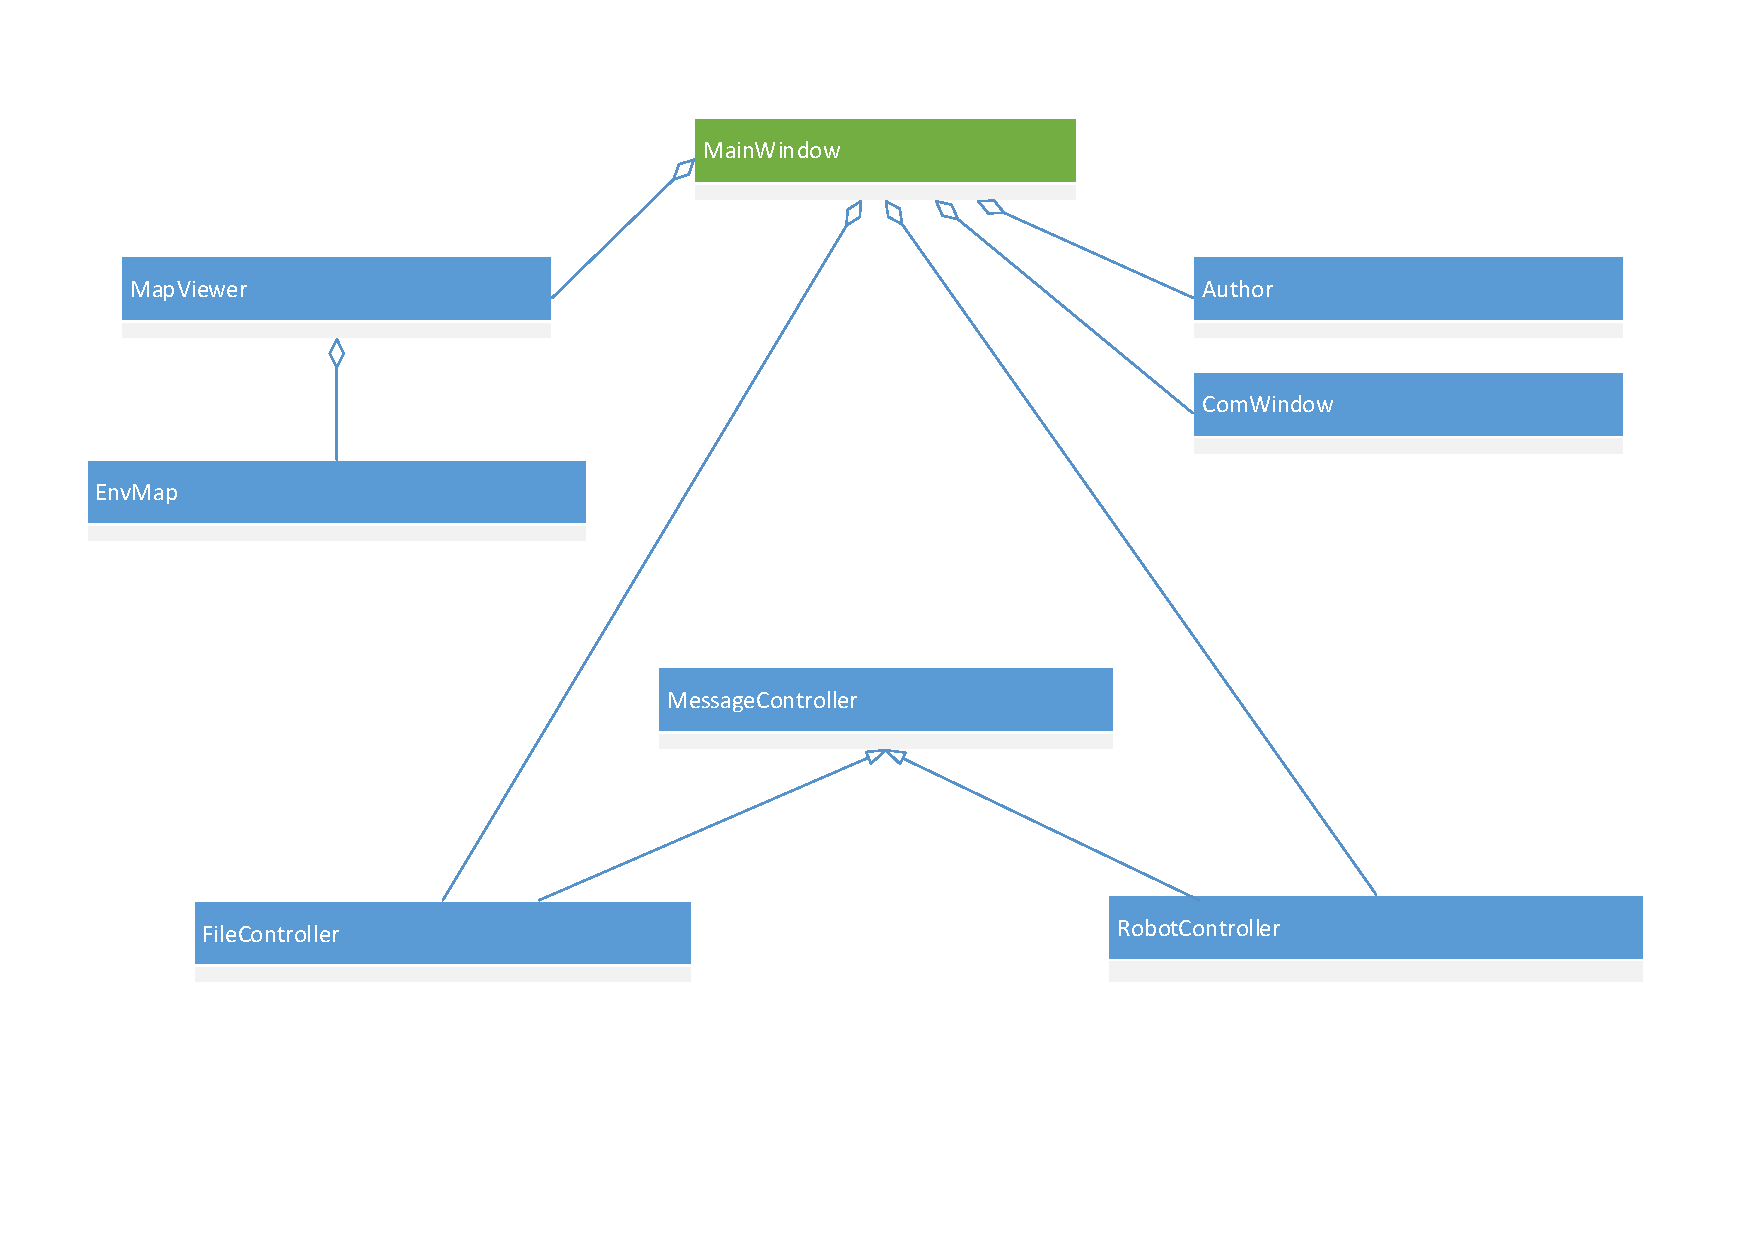
\includepdf[pages={1},landscape=true]{d_klas4.pdf}

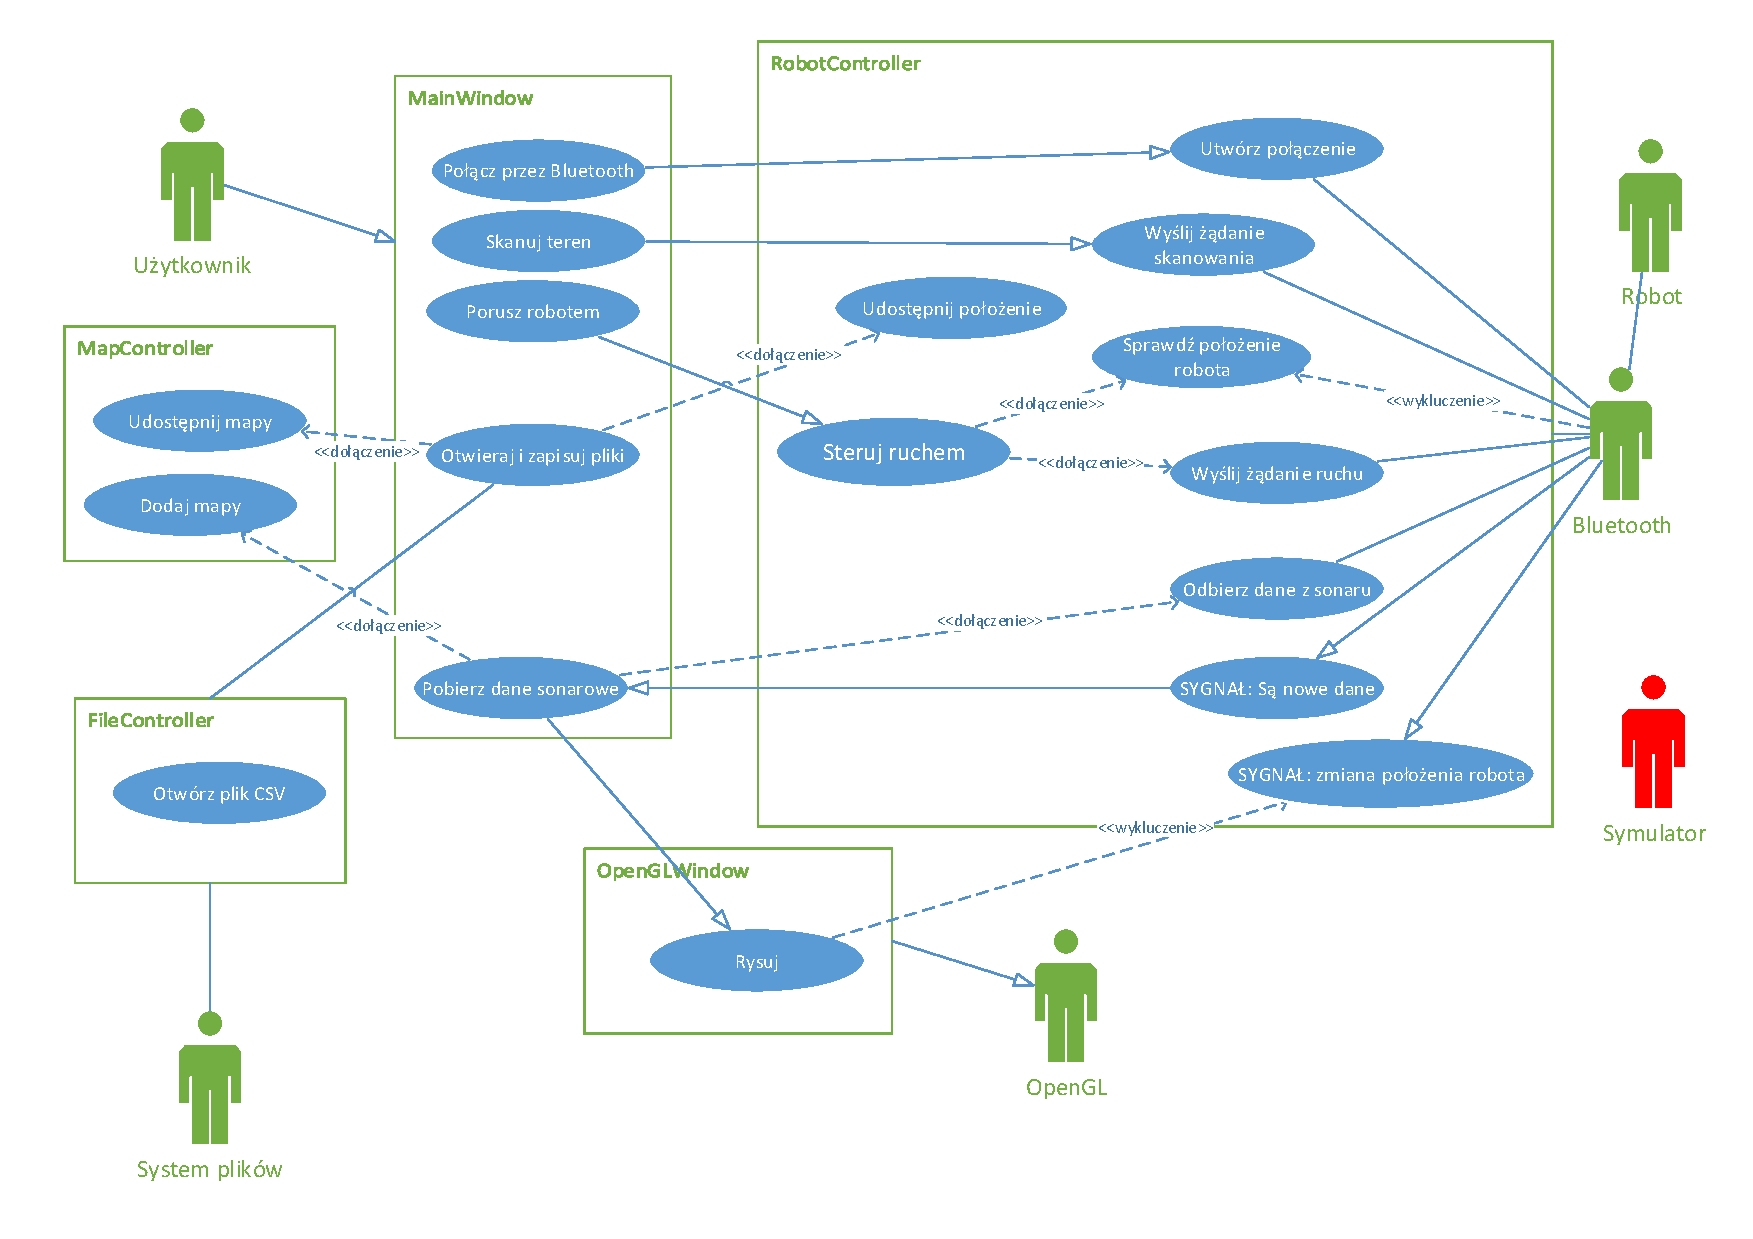
\includepdf[pages={1},landscape=true]{przypadki4.pdf}

\section{Stanowisko testowe oraz wyniki skanowania}
Kompletne stanowisko pracy składało się z laptopa, na którym tworzone były programy w odpowiednich środowiskach:
\begin{itemize}
\item aplikacja główna powstawała w środowisku Qt 5.4, przy użyciu aplikacji Qt Creator w wersji 3.3 . 
\item symulator powstawał w środowisku Android Studio 1.2 przy użyciu API w wersji 22.0.1 (Android 5.1) z kompatybilnością dla wersji 10.0.0 (Android 2.3.3 Gingerbeard).
\item program dla robota opartego na zestawie Nucleo powstawał przy użyciu systemu Keil i biblioteki mbed dla stm32f411 w programie Keil microVision5.
\end{itemize}
Na rysunku \ref{prac1} przedstawiony został fragment robota, który jest w stanie realizować funkcję skanowania otoczenia oraz symulować przemieszczenie robota. 
\begin{figure}[p]
\centering
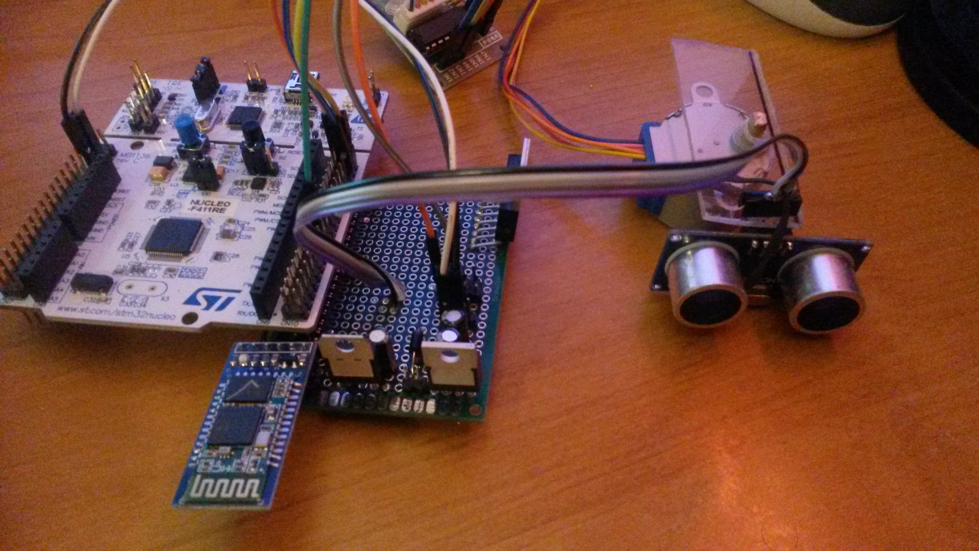
\includegraphics[width=\textheight, angle=90]{prac1.jpg}
\caption{Fragment robota}
\label{prac1}
\end{figure}

Na rysunku \ref{prac2} przedstawione zostało natomiast całe stanowisko pracy przy użyciu którego realizowany był projekt. Widać na nim robota, telefon z uruchomionym symulatorem oraz laptopa, na którym znajduje się aplikacja główna. 
\begin{figure}[p]
\centering
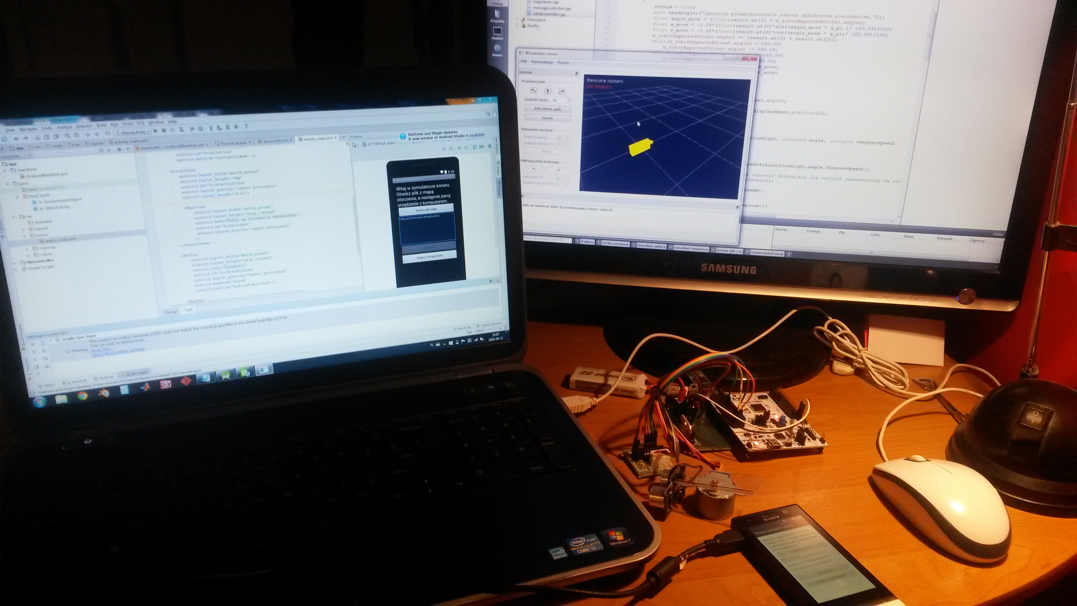
\includegraphics[width=\textheight, angle=90]{prac2.jpg}
\caption{Stanowisko pracy}
\label{prac2}
\end{figure}

\subsection{Skanowanie mieszkania}
W ramach testu przeprowadzone zostało skanowanie mieszkania. Przeskanowane zostały 3 pokoje. Rysunek \ref{stancjac} przedstawia wynik skanowania. Bez znajomości geometrii pomieszczeń trudno wywnioskować jak wygląda pomieszczenie na podstawie samego skanu sonaru. Rysunek \ref{stancjad} przedstawia ten sam wynik skanowania z naniesionymi dodatkowo informacjami nt. geometrii pomieszczeń. Jak widać wynik okazuje się całkiem zbieżny z rzeczywistą geometrią. Należy również zauważyć, że przesuwanie robota mogło nanieść spore błędy na wynik skanu. 
\begin{figure}[p]
\centering
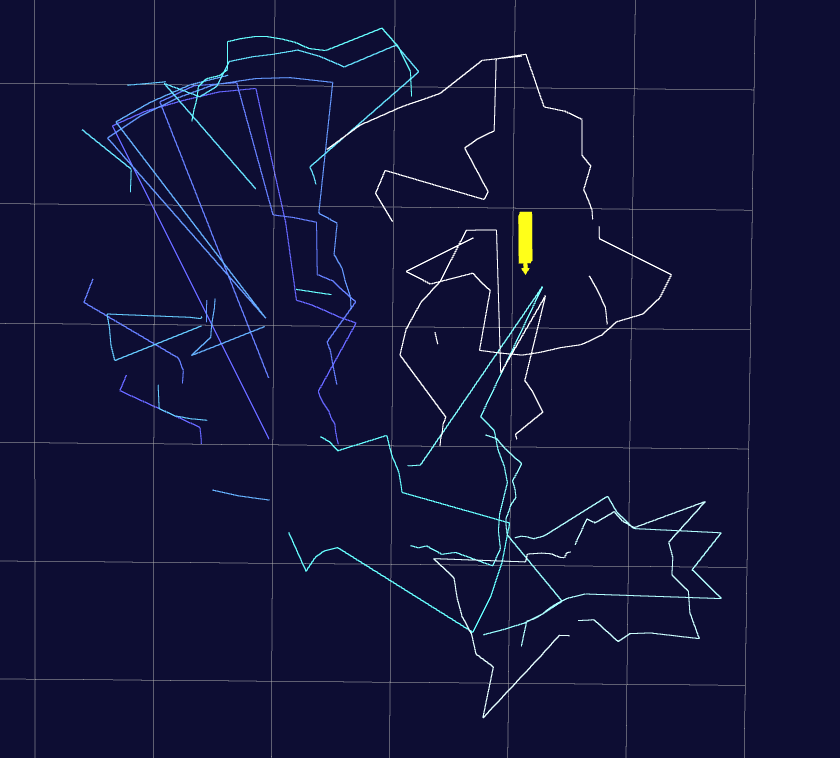
\includegraphics[width=\linewidth]{stancjac.png}
\caption{Wynik skanowania}
\label{stancjac}
\end{figure}
\begin{figure}[p]
\centering
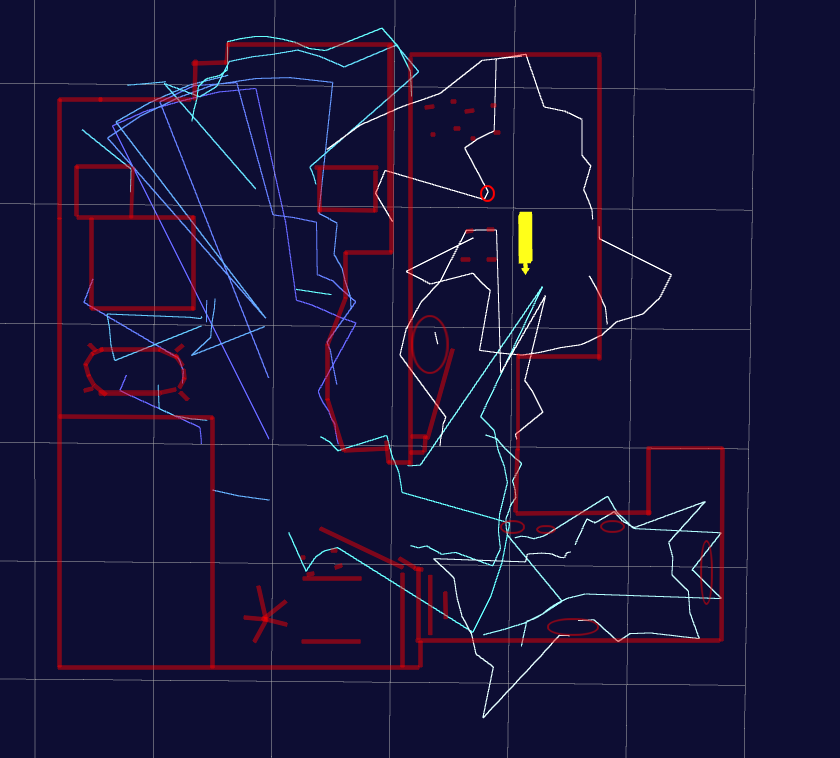
\includegraphics[width=\linewidth]{stancjad.png}
\caption{Wynik skanowania z naniesioną geometrią pomieszczeń}
\label{stancjad}
\end{figure}

\section{Podsumowanie}
Projektu nie udało się całkowicie zrealizować tak jak było to od początku zaplanowane. Nie powstał w pełni żaden symulator, który pozwalałby na pracę aplikacji bez robota. Głównym powodem takiego stanu rzeczy było nie przetestowanie możliwości zaimplementowanie połączenia bezprzewodowego. Wnioskiem na przyszłość w tej sytuacji jest to, że zanim rozpocznie się zaawansowane prace nad aplikacją należałoby najpierw wykonać testy skupione na temacie połączeń sieciowych. \newline
Odnośnie samej aplikacji komputerowej - spełniła ona wszystkie założenia, a w sumie nawet więcej niż to było zakładane przed rozpoczęciem realizacji projektu. Dodana została możliwość wyświetlania logów, kalibracji silnika czy też konfiguracji połączenia szeregowego. Należałoby jedynie w niej poprawić komunikację poprzez port szeregowy, aby odbywała się ona na osobnym wątku, ponieważ oczekiwanie na odpowiedź robota blokuje interfejs. \newline
Symulator nie jest w stanie komunikować się z aplikacją komputerową. Zaimplementowany został jednak pełny algorytm potrafiący zasymulować działanie czujnika odległościowego. \newline
Głównym problemem niezaimplementowania do końca funkcji połączenia z symulatorem były ograniczenia czasowe. 
\subsection{Subiektywna ocena}
Projekt spełnił moje oczekiwania. Brakuje symulatora, który przydałby się tymbardziej, że robot zostanie zdemontowany przez co nie uda się wykorzystać potencjału aplikacji. W ramach projektu zrealizowałem kilka celów, które sobie narzuciłem:
\begin{itemize}
\item Stworzyć aplikację, która będzie korzystała z biblioteki OpenGL - grafika 3D to jedno z moich głównych zainteresowań i projekt pozwolił mi zagłębić się w tajniki grafiki generowanej w czasie rzeczywistym.
\item Zapoznać się z zasadą działania sonaru i wynikami otrzymywanymi z takiego skanera
\item Stworzyć stosunkowo łatwą w rozwoju aplikację - jest to moja pierwsza aplikacja, która przed rozpoczęciem tworzenia została w całości zaprojektowana. Dopiero na późniejszych etapach projekt był modyfikowany, ale ogólna koncepcja pozostawała taka sama.
\item Zapoznać się z tworzeniem aplikacji na system Android.
\end{itemize}
Problemem jednak było to, że wszystkie te cele, które sobie narzuciłem były realizowane w ramach jednego projektu, przez co nie udało mi się ukończyć całości projektu w trakcie semestru. Oznacza to, że podejmując się następnych projektów powinienem ostrożniej narzucać sobie wymagania oraz szacować czas potrzebny na realizację zadań. 
\end{document}

